\chapter{Eksperymenty}
W ramach testów kontrolera przygotowałem kilka zestawów ustawień. W tym rozdziale opiszę, jak zaprojektowana przeze mnie sztuczna inteligencja radzi sobie w różnych środowiskach.

Parametry algorytmu uczącego były dobierane do wymyślonych ustawień świata w sposób eksperymentalny. Ostateczne pliki ustawień uwzględnione w tej pracy zawierają najlepsze z wypróbowanych parametrów.

\section{Ustawienia \textit{simple\_mk1} i \textit{simple\_mk0}}
Te ustawienia tworzą dość prosty świat - osiołek może zadomowić się w pobliżu jednego ostu i odżywiać się nim w nieskończoność, bo w żadnej turze nie zużywa więcej energii, niż najmniejszy możliwy przyrost masy rośliny. I do takiej właśnie strategii dochodzi za każdym razem kontroler \textit{Mark1}.
\begin{figure}[H]
    \centering
    Stan żołądka osiołka względem liczby tur poświęconych na uczenie AI
    \\(częstotliwość próbkowania: raz na 500 tur oraz przy każdym zgonie)
    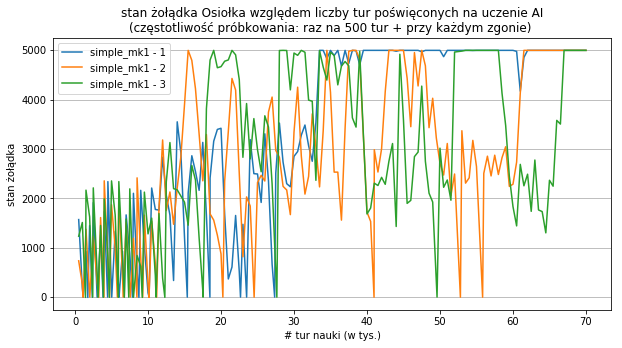
\includegraphics[scale=0.6]{Chapters/simple_mk1_hunger}
\end{figure}

Na wykresie narysowane są trzy łamane odpowiadające trzem różnym uruchomieniom programu z tymi samymi ustawieniami. Każda z nich reprezentuje w istocie wiele instancji osiołka - w momencie osiągnięcia zera symulacja resetuje się, ale kontroler zachowuje wyniesione doświadczenia. 

Z rysunku można wywnioskować, że różne uruchomienia dochodzą do strategii optymalnej w różnym czasie. Mimo to można dostrzec, że z upływem czasu zagęszczenie zgonów się zmniejsza, a wykres zaczyna oscylować w okolicach wyższych wartości. Podobne wnioski można odnieść przy wszystkich innych ustawieniach, więc dla czytelności w następnych wykresach przedstawiał będę tylko dwa uruchomienia.

\begin{figure}[H]
    \centering    
    Stan żołądka osiołka względem liczby tur poświęconych na uczenie AI
    \\(częstotliwość próbkowania: raz na 500 tur oraz przy każdym zgonie)
    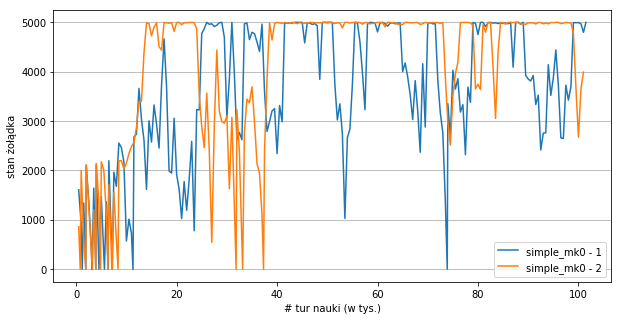
\includegraphics[scale=0.6]{Chapters/simple_mk0_hunger}
\end{figure}

Ten wykres przedstawia dwa uruchomienia z tymi samymi ustawieniami świata dla kontrolera \textit{Mark0}. Ze względu na fakt, że kontroler ten nie analizuje ostów znajdujących się poza zasięgiem interakcji nie dochodzi on do dokładnie tego samego stanu, co \textit{Mark1}. Świat budowany przez te ustawienia nie ma dużego zagęszczenia roślin. Oznacza to, że częstokroć gdy błądzący osiołek w końcu natrafia na jedną zjada ją w całości.

Mimo ograniczeń kontrolera, w każdej próbie uruchomienia programu na tych ustawieniach osiąga on stan, w którym osiołek już więcej nie umiera.

\section{Ustawienia \textit{smallStomach\_mk1} i \textit{smallStomach\_mk0}}
W przypadku tych  ustawień osiołek ma mało czasu na znalezienie pożywienia ze względu na mały rozmiar żołądka i relatywnie duże zużycie energii na turę. Utrudnia to kontrolerowi uczenie się, jednak i tu osiągana jest w pewnym momencie strategia pozwalająca na przeżycie w nieskończoność.

Sprawę ułatwia fakt, że osiołek nigdy nie zjada żadnej rośliny w całości - każda odrasta szybciej, niż ten jest w stanie absorbować jej masę, więc strategia z ustawień \textit{simple} wciąż jest adekwatna.

\begin{figure}[H]
    \centering
    
    Stan żołądka osiołka względem liczby tur poświęconych na uczenie AI
    \\(częstotliwość próbkowania: raz na 700 tur oraz przy każdym zgonie)
    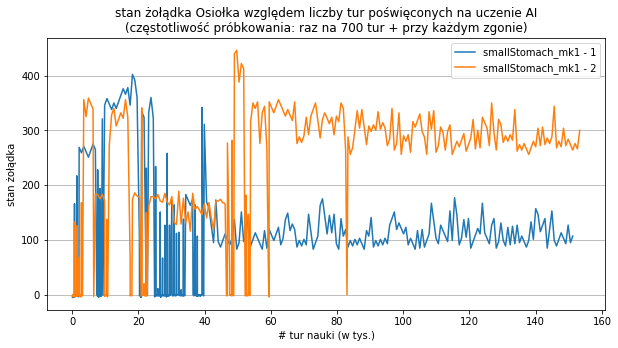
\includegraphics[scale=0.6]{Chapters/smallStomach_mk1_hunger}
\end{figure}

Choć na wykresie można dostrzec trochę mniejsze zagęszczenie zgonów wraz z postępem nauki, kontroler \textit{Mark1} daje wiele podobnie mało satysfakcjonujących żywotów i ostatni, w którym stosuje już efektywną strategię.

Ciekawym jest, że w przeciwieństwie do ustawień \textit{simple} stan żołądka po osiągnięciu stanu ostatecznego może oscylować wokół różnych wartości zależnie od uruchomienia.

\begin{figure}[H]
    \centering
    Stan żołądka osiołka względem liczby tur poświęconych na uczenie AI
    \\(częstotliwość próbkowania: raz na 700 tur oraz przy każdym zgonie)
    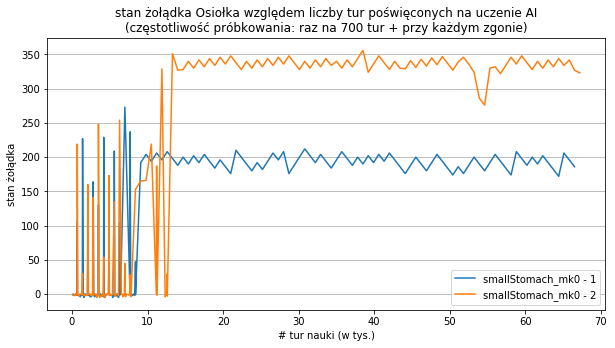
\includegraphics[scale=0.6]{Chapters/smallStomach_mk0_hunger}
\end{figure}

Podobnie jak w przypadku\textit{Mark1}, testy kontrolera \textit{Mark0} nie wykazały dużej tendencji wzrostowej w jakości strategii względem czasu, aż do osiągnięcia strategii pozwalającej na nieśmiertelność. Także i on zależnie od uruchomienia osiąga stany, w których stan żołądka oscyluje wokół różnych wartości.

\textit{Mark0} osiąga jednak strategię efektywną znacznie szybciej - mniejsza liczba rozróżnianych stanów wydaje się być w przypadku tych ustawień zaletą. Analizowanie odległych roślin nie przynosi tu korzyści, za to zwiększa czas potrzebny na naukę.

\section{Ustawienia \textit{oneBite\_mk1}}
To najtrudniejsze z przygotowanych przeze mnie ustawień. Wszystkie rośliny mają jednakową masę, wystarczająco małą by osiołek mógł zjeść je w jednej turze i nie regenerują się. Oznacza to, że zjedzenie rośliny często prowadzi do mało korzystnego stanu, w którym trzeba się przemieścić, by znaleźć kolejną. Trudno zatem znaleźć odpowiednie parametry -- mały \textbf{Discount} prowadzi do kontrolera, który preferuje się nie przemieszczać, zaś duży zmniejsza atrakcyjność jedzenia.

Spośród wszystkich sprawdzonych ustawień \textit{oneBite} daje, po nauczeniu, najciekawszy do obserwowania kontroler, ponieważ zasady świata zmuszają go do nauczenia się, jak radzić sobie w zmiennym środowisku i systematycznie odnajdywać nowe źródła pożywienia, gdy dotychczas wykorzystywane się wyczerpią.
\begin{figure}[H]
    \centering
    Stan żołądka osiołka względem liczby tur poświęconych na uczenie AI
    \\(częstotliwość próbkowania: raz na 1000 tur oraz przy każdym zgonie)
    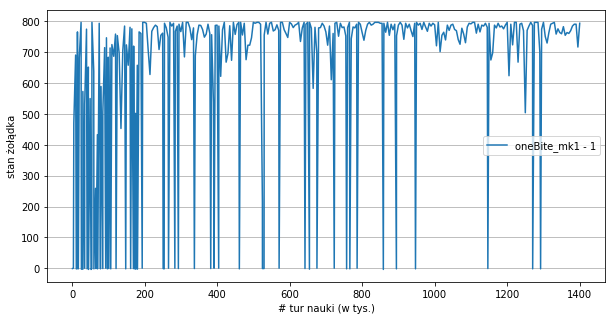
\includegraphics[scale=0.6]{Chapters/oneBite_mk1}
\end{figure}
Tym razem wszystkie uruchomienia dają bardzo podobne wykresy, więc dla czytelności przedstawione zostało tylko jedno. Można dostrzec mniejsze zagęszczenie zgonów wraz z czasem nauki, co sugeruje dążenie do efektywnej strategii. Mimo to w żadnym z wykonanych przeze mnie testów najdłuższy zarejestrowany żywot nie przekraczał 400 tysięcy tur.

Kontroler \textit{Mark0} nie daje dla ustawień \textit{oneBite} satysfakcjonujących wyników - żaden zarejestrowany przeze mnie żywot nie przekroczył 100 tysięcy tur, a zagęszczenie zgonów w czasie nie maleje z czasem.
